\commanu{ sur le titre: très clair mais un peu long avec des mots inutiles pour un titre (idem anglais): Incertitude pour la reconstruction 3D satellite, par exemple pour faire l'inverse trop court mais plus direct. bref  peser chaque mot pour avoir un titre un plus direct ?}

\chapter*{Remerciements}\addcontentsline{toc}{chapter}{Remerciements}

\newpage
\chapter*{Résumé}\addcontentsline{toc}{chapter}{Résumé}

\newpage
\chapter*{Abstract}\addcontentsline{toc}{chapter}{Abstract}

\newpage
\vspace*{\fill} 
\begin{quote}
\vspace{1cm}
\centering
``\textit{You never talk of likelihoods on Arrakis. You speak only of possibilities.}''
\end{quote}
\vspace{0.5cm}
\begin{flushright}
Frank Herbert, \textit{Dune}
\end{flushright}
\vspace*{\fill}


\newpage
\chapter*{Introduction}\addcontentsline{toc}{chapter}{Introduction}
Knowing the Earth's topography is crucial for modern geosciences. Depending on the level of details needed, different models can be used: the Earth ellipsoid, its geoid (gravity equipotential surface), contour lines on hiking maps \etc One of those models is the \acrfull{dsm}, which is a representation of a surface's elevation on a regular grid. This type of model appears as a natural solution in many \acrfull{gis}. Indeed, they can easily be handled and provide georeferenced information regarding the topography of an area. \Cref{fig:intro_dsm_example} presents an example of a DSM\commanue{A voir si c'est ici que tu mets la différence entre DSM et DTM. Avec le fait que le DSM tient compte du sursol donc parfois en fonction des applis il faut passer par un DTM.}.

\acrshort{dsm}\commanue{Je trouve cela un peu bizarre de considérer DSM au pluriel. En plus c'est pour en parler de manière générique. Tu peux laisser au singulier. Après si tu veux vraiment le pluriel, perso je mettrais DSMs} find usage in various contexts and for a wide range of applications. In \acrfull{eo} for instance, \acrshort{dsm} are used to monitor changes in vegetation \cite{sadeghi_canopy_2016}, melting rates of glaciers \cite{berthier_glacier_2014, rieg_pleiades_2018}, volcanos \cite{ganci_data_2022}, snow or water resources \cite{marti_mapping_2016, gascoin_theia_2019, yamazaki_merit_2019} \etc\commanue{alors perso je ne suis pas fan du etc mais c'est une question de goût} Similarly, \acrshort{dsm} are employed for catastrophe management, to predict the potential damage caused by earthquakes or floods \cite{jenkins_physics-based_2023} \etc\commanue{vu que tu n'as qu'un seul exemple je ne mettrais pas le etc} \acrshort{dsm} are also crucial for ortho-rectifying images, \ie geometrically correcting the effects of distortions between the sensor and the terrain\commanue{si on voulait être plus précis on pourrait dire effects of distortion due to the sensor's angle of view and the terrain's relief}. This process creates a planimetric image with a consistent scale in all parts of the image. It allows images to be easily used in GIS or as background for maps. Finally, high resolution \acrshort{dsm} can help drone navigation in urban settings, for Defense applications, or more broadly for urban planning \cite{velazco_3d_2012}.

\begin{figure}
    \centering
    \begin{subfigure}[t]{0.5\linewidth}
        \centering
        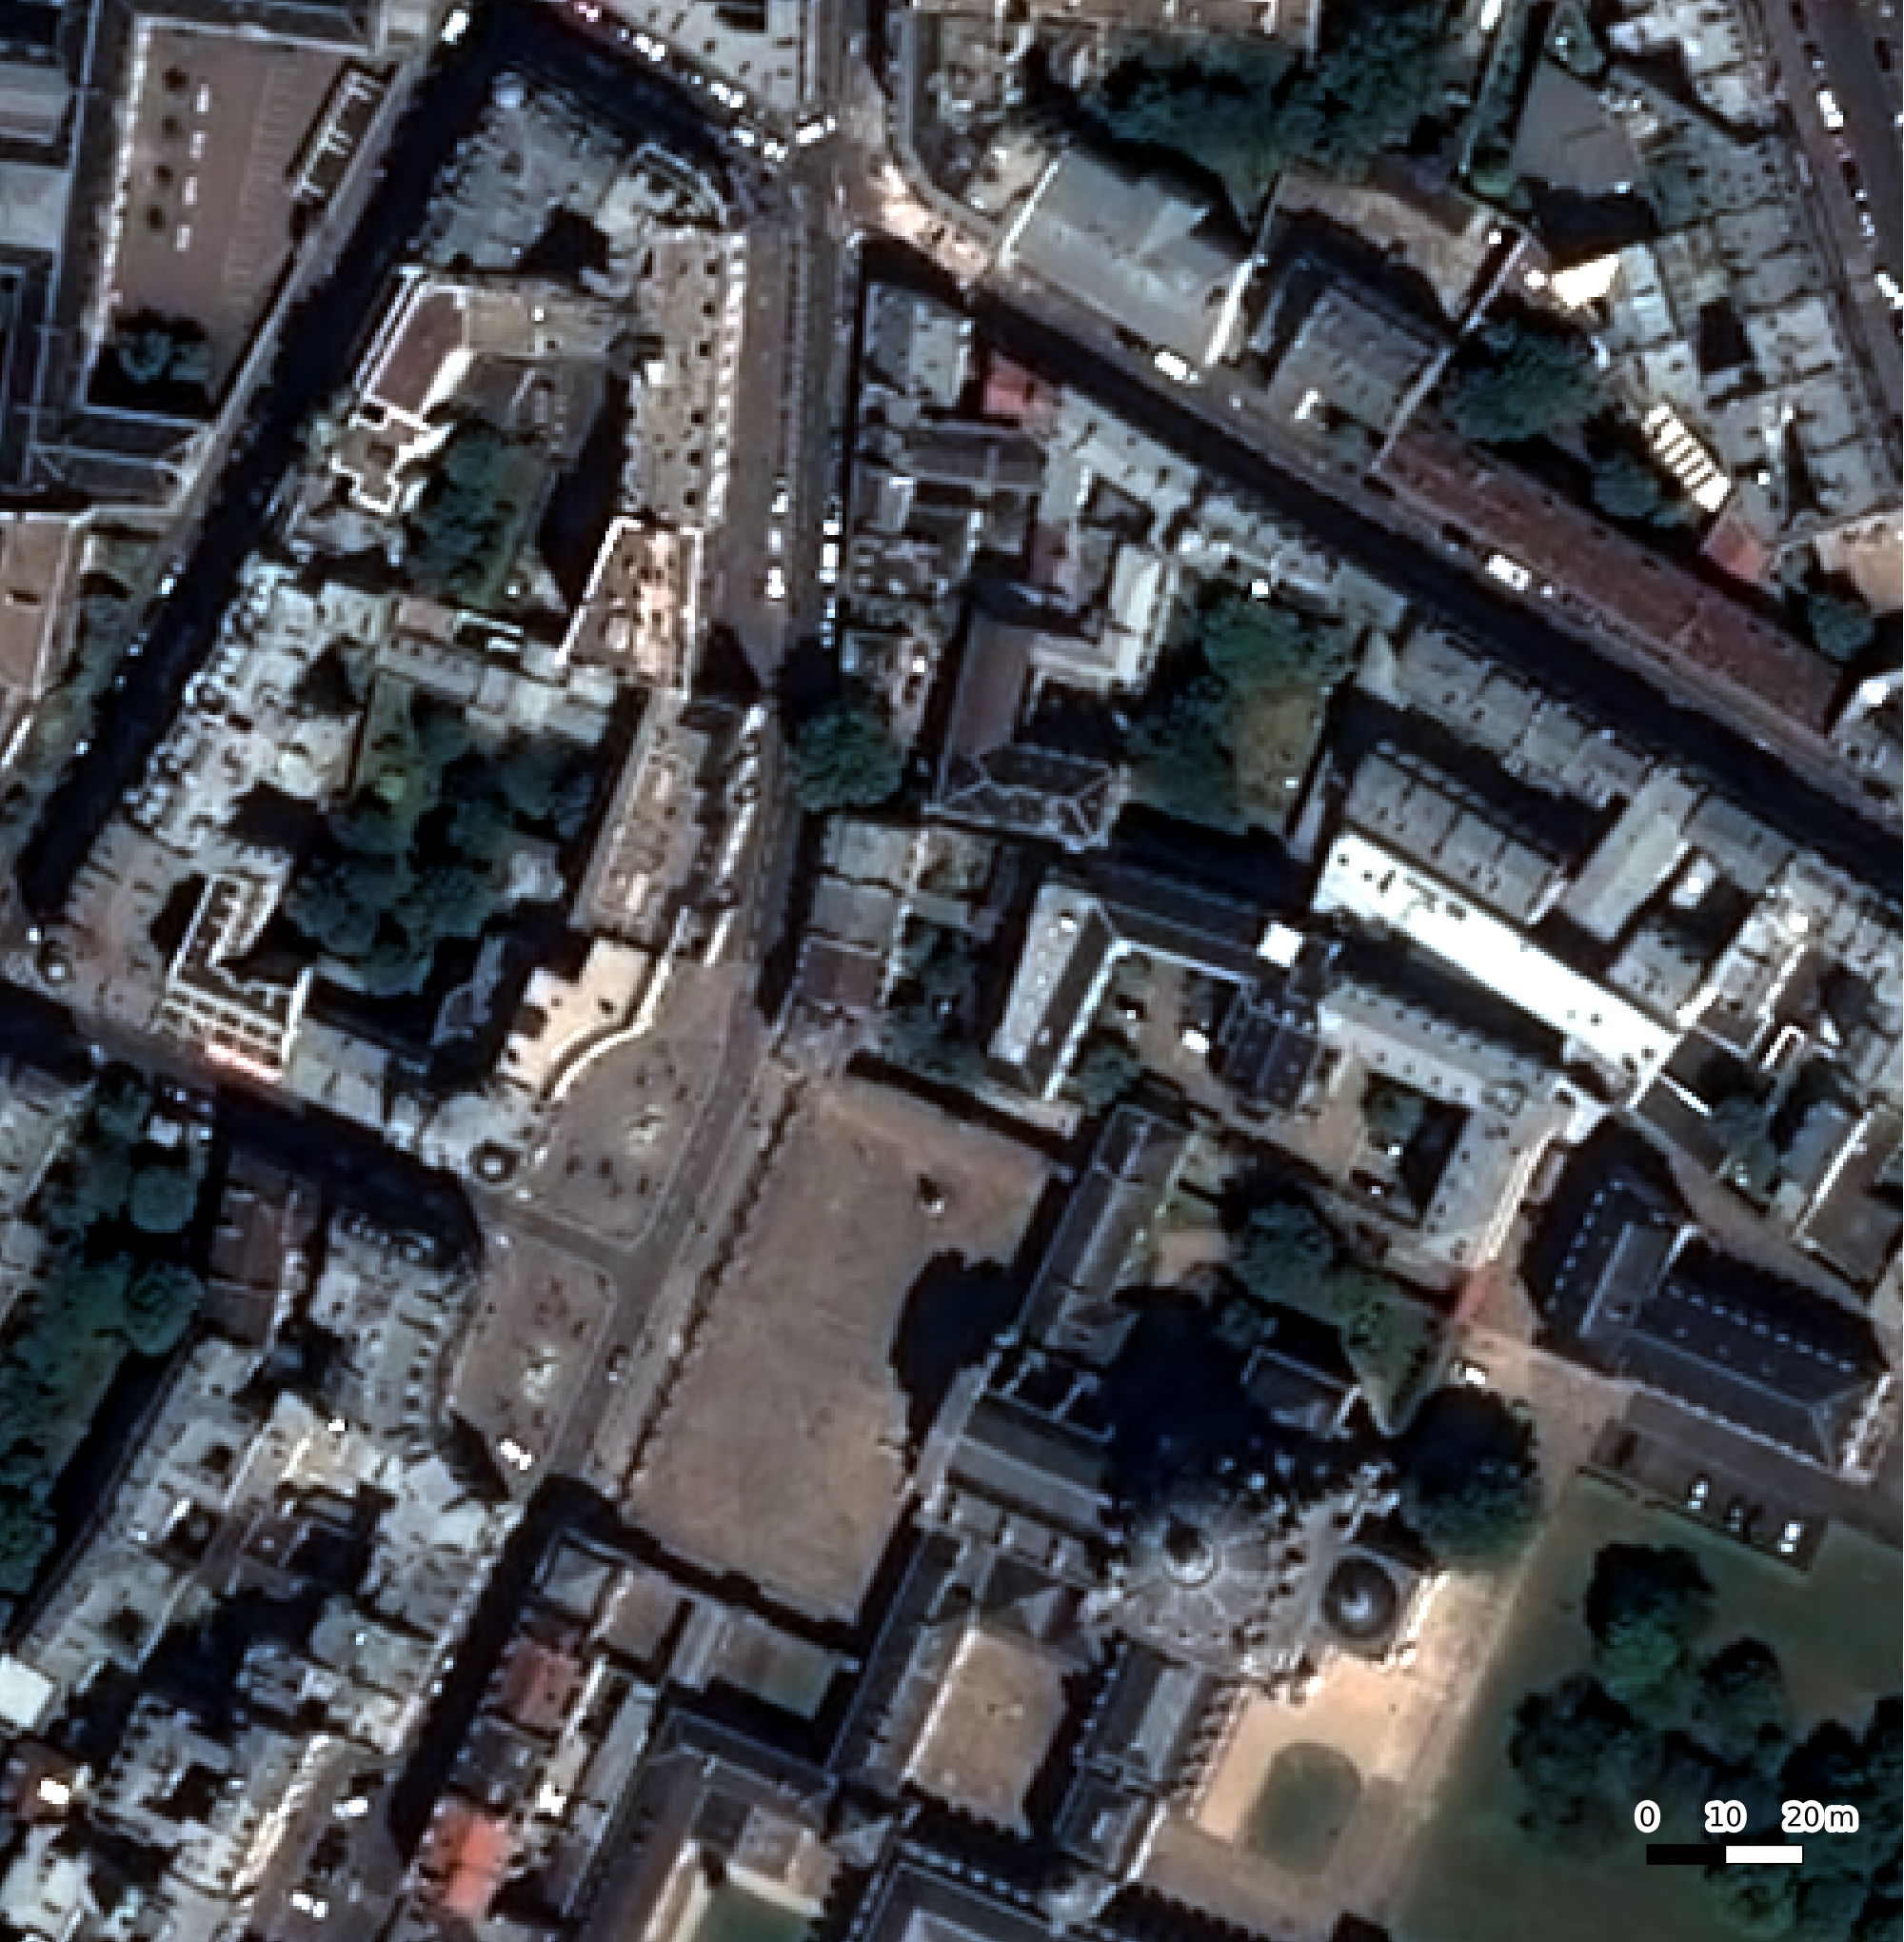
\includegraphics[height=6cm]{Images/0_Intro/Paris_Ortho.png}
        \caption{Pléiades image \copyright CNES 2017, Distribution AIRBUS DS}
        \label{fig:VDG_ortho}
    \end{subfigure}\hfill
    \begin{subfigure}[t]{0.5\linewidth}
        \centering
        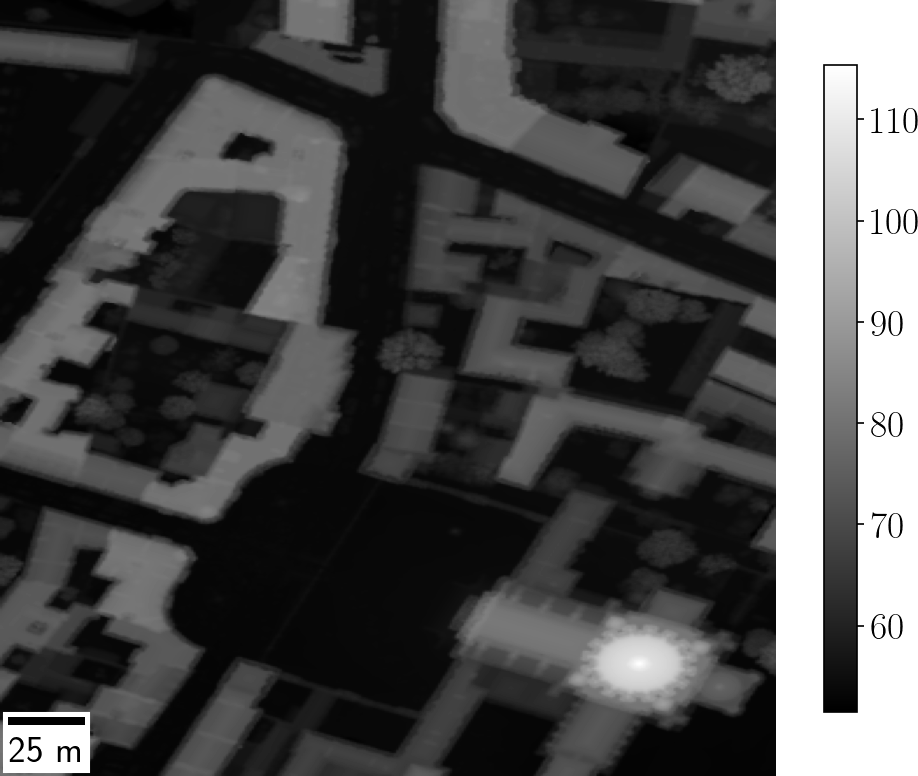
\includegraphics[height=6cm]{Images/0_Intro/Paris_DSM.png}
        \caption{Digital Surface Model from LiDAR HD}
        \label{fig:VDG_dsm}
    \end{subfigure}
    \caption{Satellite image over Val-de-Grâce, Paris at $0.5$m of resolution, and a DSM over the same area.}
    \label{fig:intro_dsm_example}
\end{figure}

There are multiple ways of creating a DSM\commanue{Alors dans ce qui suit tu te limites aux solutions aéroportées (avion ou drone) et satellites qui permettent de des DSM sur des zones assez étendues.}. The first way\commanue{je ne sais pas pour l'ordre tu commences par le satellite SAR qui est de l'ordre de 10m pour TerraSAR/TandemX au mieux pour les produits récents, tu passes par le lidar qui est un radar mais pas interféromètre qui est plutôt de l'ordre < 1m et ensuite tu reviens au satellite optique cette fois. Mais tu ne compares pas le SAR avec l'optique. Il faudrait aussi donner un ordre de grandeur de la précision alti. Tu te limites à la résolution.Comme on parle de DSM si tu ne souhaites pas parler de la précision alti que tu n'as pas forcément, tu pourrais donner come indication le niveau de détail visible dans les produits (par ex est-ce qu'on duisngue les bâtiments). Ainsi le SRTM peut être échantilloné à 30m, on distingue quand même pas grand chose sur les villes. Avoir si tu mets cette info en intro ou dans le chapiter 1} is to use radar interferometry, as done by Sentinel-1 satellites \cite{geudtner_sentinel-1_2014} or the Shuttle Radar Topography Mission (SRTM) \cite{farr_shuttle_2007}. This method presents the advantage of being able to acquire data by day and night, even in the presence of clouds. Typical resolutions obtained are in the range of a few meters. For instances, the worldwide DSM produced by the SRTM mission has a resolution of $30m$. An other method for producing DSM are using LiDAR (laser sensors) \cite{khosravipour_generating_2016}. Using those sensors allows to obtain very good accuracy. For instance, the french institude IGN (\textit{Institut national de l'information Géographique et forestière}) is using LiDAR to cover the french territory with a resolution of $10$ points per $m^2$. However acquisitions campaigns such as this one are carried out using airborne vehicles, and are thus costly and take a lot of time. Finally, it is possible to construct DSM by means of (stereo) photogrammetry \cite{tao_comprehensive_2001}\commanu{remarque minime, mais je mettrais pas de parenthese sur stereo, comme tu l'utilises ensuite après}, \ie the science of recovering 3D information from optical images. For this method, images of a scene are acquired from different points of view, and depth information is recovered from the parallax effect between images\commanue{Peut-être un schéma car tu mentionnes plusieurs fois l'effet de parallax mais c'est pas forcément évident pour qqn qui n'a pas l'habitude. Ou alors tu dis comme les yeux si tu ne souhaites pas rentrer trop dans les détails}. As current optical satellites have a sub-meter resolution, it is possible to massively produce DSM covering the globe using photogrammetry for a relatively low cost\commanue{Là encore quand on est pas du domaine, si les satellites prennent des images submétriques on peut espérer des DSM à quelle résolution et à quelle précision ou plutôt quel niveau de détail/éléments}. Throughout this thesis, we will mainly consider photogrammetry as our mean\commanue{c'est bizarre en anglais donc method/approach/autre choix} to produce DSM.

In this context, CNES - the French Space Agency - is planning to launch 4 low-cost optical satellites with Airbus Defense and Space, in order to massively produce DSM using stereo photogrammetry. This mission, named CO3D (for \textit{Constellation Optique 3D}, \cite{melet_co3d_2020}), was conceived jointly with IGN to provide high resolution DSM over the globe, at a $50cm$ resolution.

CNES also\commanue{alors je ne suis pas fan de la transition, je mettrais plutôt For this purpose, CNES developed...}\commanu{tout à fait d'accord} developed a pipeline dedicated to process all images provided by the CO3D satellites automatically and at a very large scale. This pipeline is called CARS (``Chaine Automatique de Restitution par Stéréoscopie''), and is composed of many different image processing algorithms\commanue{je mettrais juste many processing steps}. As stated previously\commanue{on est dans l'intro donc tu as mentionné rapidement le principe du pipeeline mais c'est tout. En fait tu as remonté ce parapgraphe du chapitre 1. A mon avis il faut retravailler la fin du paragraphe. Tu n'as pas besoin de rentrer dans les détails. Tu peux peut-être juste dire que le pipeline sera détaillé dans la suite et que dans cette thèse tu te focalises sur une des étapes principales qui est le stéréo matching. Je pense qu'il te manque une phrase dans le genre.}, the depth information is retrieved from the parallax effect between images, \ie the different movement of objects in-between images depending on their distance to the sensors\commanue{donc c'est maintenant que tu définis la parallax alors que tu l'utilises avant donc peut-être à remonter}. The quantification of this movement is done during a step called dense-matching, where we try to find the different positions of each pixel in multiple images. Dense-matching is therefore the core part of the CARS pipeline, and it is also a popular problem in computer vision in general (for autonomous cars for instance \cite{geiger_are_2012}) \commanu{d'accord avec remarques de manue sur le chapitre à revoir, sur trop de détails à ce niveau et le parallax}.

Alongside DSM\commanue{peut-être ajouter computation}, one of the requirements of the CO3D mission is to produce a performance map indicating the estimated quality of each cell of the DSM. This motivated\commanue{bon alors je ne sais pas pour le temps au passé. En général je ne suis pas fan quand on mélange les temps dans un paragraphe.}\commanu{idem, j'aime pas trop la transition et le temps, je propose plus direct: Given the limited state-of-the-art on the subject, this motivates CNES to lead research to the issue of uncertainty in the CARS pipeline.} CNES to lead research which investigated the uncertainty amongst the CARS pipeline. The main objective of this thesis was to\commanue{le mot 'to' est en trop je pense}\commanu{+1 et mettre au présent -> is} therefore to characterize and propagate the uncertainty throughout this photogrammetry pipeline. However, it was clear from the beginning that characterizing the uncertainty of every step of the pipeline was too much work one thesis\commanue{alors oui c'est vrai mais c'est pas top comme tournure. En français je dirais un truc du genre : afin d'obtenir des résultats qui pourraient être implémenté avec les contraintes planning du segment-sol, cette thèse s'est focalisée sur l'étape de stéréo matching qui est la source des erreurs.}\commanu{+1, trop négatif dès le début à dire qu'on fera pas tout, bcp mieux la tournure de manue en intro}, as many complex algorithms interact inside CARS. We thus mainly focused\commanu{donc focus au présent} in the dense-matching step: being the crucial and hardest part of the pipeline, it is also the step that is the most determining for the final uncertainty\commanue{A mon avis, il faut retravailler les deux paragraphes (celui là et le précédent), tu as des redites}.

\commanue{Bonne intro sur l'incertitude, bravo !}\commanu{en effet}
As we will deal with uncertainty throughout this thesis\commanue{proposition de transition: Before delving into uncertainty estimation and propagation through this thesis}, we first need to specify what we mean by uncertainty. Uncertainty is a situation where a measure or value of interest is not known, or not known with precision. It is subject to change, as additional information, measures or a different acquisition protocol may reduce how uncertain a value is. It can also be subjective. For instance, someone may be uncertain about the launch date of CO3D satellites while someone else working at the launch pad might have the answer. This highlights the fact that while everyone has an understanding of what uncertainty is, it encompasses very different concepts in nature. It is common to differentiate the various types of uncertainty by dividing it into two categories: stochastic (or random) uncertainty and epistemic uncertainty.

Stochastic uncertainty refers to every situation of purely aleatoric nature. For instance, the result of a coin throw, random noise on a CCD captor or the Brownian movement of a particle. An operator typically encounters this kind of uncertainty in a situation where they have\commanue{si c'est an operator c'est he qu'il faut mettre et pas they} access to many measures or observations of the same value of interest. It is usually modeled mathematically with a frequentist approach, using probability measures such as the uniform distribution, Gaussian distribution, Student's $t$ distribution \etc \commanu{j'enleverais l'etc, je trouve que attention dans une intro à l'utiliser vraiment quand nécessaire. Ici tu n'as pas besoin (such as)}

On the other hand, epistemic uncertainty refers to a situation where the value of interest is not known or ill-known due to a lack of knowledge. Think of the previous example with the launch date of satellites, or if someone was asked to guess Io's mass, one of the moons of Jupiter. There is no random process at stake here, and there is usually no point of acquiring multiple samples of the measure. Once the value of interest is known, the uncertainty usually no longer exists. It has been proposed to model this kind of uncertainty using a Bayesian approach for probability, by opposition with the frequentist approach. Probabilities here represent a state of knowledge, or degree of belief, one has over the value of interest. It can be updated with additional knowledge, thus leading to the notion of prior and posterior probabilities. We will see during this thesis that other model can be used to characterize this uncertainty, for instance \textit{imprecise probabilities} and more specifically \textit{possibility distributions}. It is note the first time\commanue{It is worth noting that this is the first time that} that those models are considered for processing satellite imagery, as another thesis estimated land changes uncertainty using possibility distributions\commanue{j'ai un doute sur ta phrase ou c'est mon anglais qui est mauvais}\commanu{idem je comprends pas si c'est bien la première fois ou pas vu ton argument. Si il y a une autre citation et ce n'est pas la première fois, tu peux tourner en disant : au mieux de notre connaissance, l'utilisation des probas imprécises dans notre contexte est dans les premiers travaux, avec ... et tu cites. Bref, pas négativement dans l'intro} \cite{lesniewska-choquet_specialite_2020}.

Although uncertainty can be complex and expensive to compute\commanu{mais peut etre optionnel... je mettrais pas ca en "négatif" dès le début meme si c'est vrai, par exemple. Uncertainainty characterisation and quantification have several benefits, despite the obvious complexity and computation cost }, characterizing and quantifying it has many benefits. It provides \commanu{indeed} additional information for better decision making and risk management. It can also allow for a better understanding of the underlying processes at stake regarding the value of interest. In many cases, uncertainty estimation is treated as a secondary objective in applications. However, jointly estimating a value and its uncertainty can lead to new strategies to reduce the uncertainty or sometimes even improve the performances of the main applications \cite{chen_learning_2023,jiang_unsupervised_2024}\commanue{je mettrais ce paragraphe plus haut car tu parles ici de l'incertitude au sens large.}.

During this thesis, we\commanue{Je viens de remarquer le pronom we. Je ne sais pas si tu l'utilises avant. Vois avec Seb car je ne sais pas si maintenant il faut mettre nous ou je. Dans les rapports de stage, ils préfèrent je mais pour un manuscrit de thèse je ne sais pas}\commanu{mon avis: mettre je en effet, c'est ta thèse, et je sais pas si le both se met pas après, on a l'impression que vous etes 2 à avoir contribuer avec le we -> I have contributed to both the field ... and the field} both contributed to the field of photogrammetry and to the field of imprecise probabilities. Here is a quick overview of the contents that can be found in the following chapters:
\begin{itemize}
    \item \Cref{chap:stereophotogrammetry} introduces the different stereo photogrammetry concepts considered in this thesis. It focuses on the stereo pipeline developed by CNES and its sources of uncertainty, which will be considered in our applications.
    \item \Cref{chap:representation_of_uncertainty} will introduce the different uncertainty models considered in this thesis, mainly possibility distributions and copulas. The end of \Cref{chap:representation_of_uncertainty} and the following chapters constitute the main contributions of this thesis\commanue{moi je mettrais pas cette phrase}.
    \item In \Cref{chap:joining_credal_sets}, we propose different methods for creating specific multivariate uncertainty models based on the models introduced in \Cref{chap:representation_of_uncertainty}. We also study the relationships between the methods we introduced.
    \item \Cref{chap:propagating} uses the concepts of \Cref{chap:representation_of_uncertainty} and the results of \Cref{chap:joining_credal_sets} to propagate uncertainties modeled by possibility distributions in a part of the dense-matching step of the stereo pipeline.
    \item \Cref{chap:epistemic_uncertainty} also uses possibility distributions, but this time to characterize the uncertainty of the dense-matching step itself. Using this method, we are able to obtain confidence intervals at the end of the dense-matching step. Those intervals are then propagated to the end of the pipeline, to generate confidence intervals on the final DSM.
\end{itemize}

\commanu{intéressant de guider le lecteur sur les 2 champs de compétences mais tu peux faire plus direct comme transition. Genre, tu remplaces ce petit paragraphe avec par exemple: To help readers in following chapters depending on their field of expertise, here is a classification of each chapter}
\commanu{tu pourais meme peut etre gagner sur l'intro en mergeant avec la présentation au dessus de chaque chapitre, je trouve que ca rallonge alors que tu pourrais faire quasi la meme chose en meme temps qu'au dessus, mais tu vois...}
Allow us to make a small disclaimer\commanu{effet de style qui accouche un peu d'une souris à mon avis, juste un feeling à la lecture, je mettrais pas.}: because our contributions concern two distinct fields of research, readers with a level of expertise in one field might be less interested in the second field. We tried, as much as possible, to write each chapter so it can be read and followed by everyone, although some details might need additional knowledge in a field of expertise. To help readers to navigate through chapters according to their center of interests, here is an attempt to classify each chapter into its field of research.
\begin{itemize}
    \item \Cref{chap:stereophotogrammetry} focuses on stereo photogrammetry.
    \item Chapters \ref{chap:representation_of_uncertainty} and \ref{chap:joining_credal_sets} focuses on the modelling of uncertainty.
    \item \Cref{chap:propagating} joins both fields, but leans a bit more towards uncertainty propagation than towards photogrammetry. 
    \item \Cref{chap:epistemic_uncertainty} also attempts to join both fields of research, but focuses almost completely on photogrammetry.
\end{itemize}

\commanu{je mettrais pas cette section technique hyperref dans l'intro, en annexe si tu veux vraiment garder avec un lien, en tout cas c'est pas le but de l'intro, ca  met le lecteur ailleurs...}
\begin{remark}
    A small digression that can be helpful for navigating through this thesis on a computer. We tried to make an extensive use of the \textit{hyperref} package, so that reading this thesis on a PDF viewer was made easier. You can thus click on citations, figure numbers, equation numbers, chapters and sections number, acronyms \etc to directly jump to the concerned part. Depending on the OS of you computer and the app used to read the PDF document, there usually exist shortcuts to jump back to the previous view. This allows to quickly switch back and forth between chapters and sections. Imagine that you are in \Cref{chap:epistemic_uncertainty} and we make a reference to an equation form \Cref{chap:representation_of_uncertainty}. If you do not recall the equation, and quickly want to see what it is about, just click on the hyperlink to directly go to the relevant equation from \Cref{chap:representation_of_uncertainty}. Then use your system's shortcut to go back to where you were in \Cref{chap:epistemic_uncertainty}. 
    \begin{itemize}
        \item Using Acrobat Reader: the short cut \keys{\Altwin + \arrowkeyleft} (left arrow key) on Windows or Linux brings you to the previous view after clicking on a hyperlink. Afterwards, you can alternate views with \keys{\Altwin + \arrowkeyright} and \keys{\Altwin + \arrowkeyleft}. On MacOS, the \keys{\Altwin} key is replaced by the \keys{\cmd} key.
        \item Using Preview on MacOS, you can add the \menu{Page History} button to the toolbar, by right-clicking on the toolbar and selecting \menu{Customize Toolbar}
        \item Using Okular on Linux, \keys{\Altwin + \shift + \arrowkeyleft} (left arrow key) brings you to the previous view after clicking on a hyperlink. Afterwards, you can alternate views with \keys{\Altwin + \shift + \arrowkeyright} and \keys{\Altwin + \shift + \arrowkeyleft}
    \end{itemize}
\end{remark}

The rest of this section lists the contributions and research events that occurred during this thesis.
\commanu{j'en ferais une section non numérotée (chapter*) Publication list, Contribution list, et j'enleverai la phrase (the rest est francais si tu la gardes: the remainder of this section ..., mais sinon c'est bien cette tendance d'avoir tes contributions au début bien identifiées. + à la lecture, t'as des manques sur certains endroits trop générique notamment sur workshops, poster sessions: mets juste Oral communication et enleve le etc...}

\noindent National conferences:
\begin{itemize}
    \item LFA 2022: ``Copules, probabilités inférieures et ensembles aléatoires : comment et quand les appliquer ?''  \cite{malinowski_copules_2022}
\end{itemize}
International conferences:
\begin{itemize}
    \item SMPS 2022: ``Copulas, Lower Probabilities and Random Sets: How and When to Apply Them?'' - \cite{malinowski_copulas_2022}
    \item ISIPTA 2023 (Special jury recognition Award): ``Uncertainty Propagation using Copulas in a 3D Stereo Matching Pipeline'' -  \cite{malinowski_uncertainty_2023}
    \item IGARSS 2024: ``Robust Confidence Intervals For Digital Surface Models Using Satellite Photogrammetry'' -  \cite{malinowski_robust_2024}
\end{itemize}
International journals:
\begin{itemize}
    \item International Journal of Approximate Reasoning: ``Uncertainty propagation in stereo matching using copulas'' -  \cite{malinowski_uncertainty_2024}
\end{itemize}
Not yet published pre-print:
\begin{itemize}
    \item : Available on ArXiv: ``Robust Confidence Intervals in Stereo Matching using Possibility Theory'' - \cite{malinowski_robust_2024-1} \commanu{bizarre le : au début, remettre en forme}
\end{itemize}
Workshops, poster sessions \etc:
\begin{itemize}
    \item Belief 2022 conference: Poster presentation \commanu{a préciser, trop générique, quel titre ?}
    \item Workshop Imagin ``journée imprécision et incertitude en analyse et traitement d'images'': Funding of the event and communication. Also an oral presentation
    \item SFPT ``Pléiades Neo: de nouveaux satellites pour de nouveaux usages'': Oral presentation
    \item GdR IASIS ``Télédétection et Climat'': Oral presentation
\end{itemize}

\pagebreak
